\documentclass{article}
\usepackage{graphicx}

\title{On Learning Math}
\author{Michael Yang}

\begin{document}

\maketitle
I first learned about the area of a circle in second grade when our teacher gave it to us as a formula to use. Now, I should get one thing straight — even though I love all the beauty and ingenuity in math, I am, despite my best efforts, unfortunately not a naturally experimental mind. As a result, I was more than content to sit down and compute areas of different-sized circles without knowing why the formula was true. (Perhaps ironically, what I really took an interest in was the value of pi; this led to me memorizing many more digits of it than I will ever need.) 

In fourth grade, geometry struck again; I was introduced to the volumes of the cylinder, sphere, and cone. I vividly remember when our class measured three cones’ worth of water, then poured it all into a cylinder of the same radius and height. We were all so surprised when the volumes fit perfectly! Afterwards, many of my classmates crowded around our teacher, begging to know why it was true. Embarrassingly, I was again not one of them. “Ah,” I thought, “it’s obviously because we can somehow stack the three cones perfectly inside the cylinder! What could be more natural?” 
\begin{center}
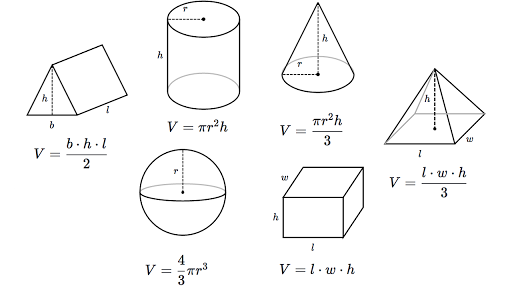
\includegraphics[scale=0.33]{images/geo_figures.png}
\end{center}
Unfortunately, I quickly learned that the answer wasn’t that simple. In middle school, I repeatedly heard that the volumes of these seemingly “easy” solids actually required something called integration, whatever that meant. And yet, I still wasn’t bothered enough to look anything up. In a repeat of my second-grade self, I was content to plug in numbers into math competition problems, pausing only to groan whenever I messed a formula up. 
\begin{center}
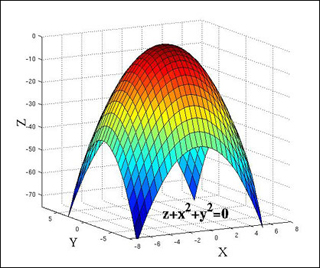
\includegraphics[scale=0.45]{Magazines/img/Vol3/multivar.jpg}
\end{center}
It was only a few months ago, when I was taking a multivariable calculus class, that I finally saw the machinery behind why these formulas are true. Our teacher presented us with a monstrous triple integral one day as a “warm-up problem” — making our dissatisfaction audibly known, our table slogged through the pages of computation. But what really surprised us was the answer: an integer multiple of pi. As it turns out, what we had actually done was to compute the volume of a cone in disguise! The cylinder and sphere quickly followed; just for fun, we did the circle, too. And thus, in that one hour, I resolved the questions which I hadn’t been willing to ponder for the past decade. 

What did I learn from all this? Well, be curious — if I had looked at the origins of these formulas earlier, I might have gotten interested in calculus and higher math long before I actually did. But I also think that there’s another point at play here: one of math history. There was a reason why we needed to appeal to triple integrals to determine the volume of a cone: the math we learn in second grade might be simple, but it’s definitely not easy. These sorts of problems stumped even the brightest minds of the Ancient Greeks; even though Archimedes almost certainly knew of these formulae, he famously lamented that he could not make his methods rigorous. It took until the late seventeenth century (almost two millennia later!) — when Newton and Leibniz introduced calculus — to make the proofs airtight. 

Math carries with it an incredible history, one that reverberates through time and space. It’s one that is truly international, with amazing math coming from every corner of the world. And, at its core, math is about collaboration. The proof of the area of a circle wasn’t found alone; neither was the volume of a sphere. The average high schooler now knows geometry unknown to Euclid and number theory unknown to Gauss not because our generation is that much better, but because we’ve been able to build off their work and the work of those that have come after them. 

Too often in the way math is first presented, the focus is on getting the answer right: you either use the formula correctly or you don’t. What too often goes unsaid is that some of the most brilliant mathematicians undoubtedly struggled proving the formula you’re using. And that’s why studying math history is so important: we can appreciate just how far we’ve come as a collective. 

So next time you encounter a formula you don’t know how to prove, ask yourself not just why, but also how, we know it’s true. Who knows? Sometime in the future, high school students may very well be solving the hardest open problems of our generation as warm-ups. 
\begin{center}
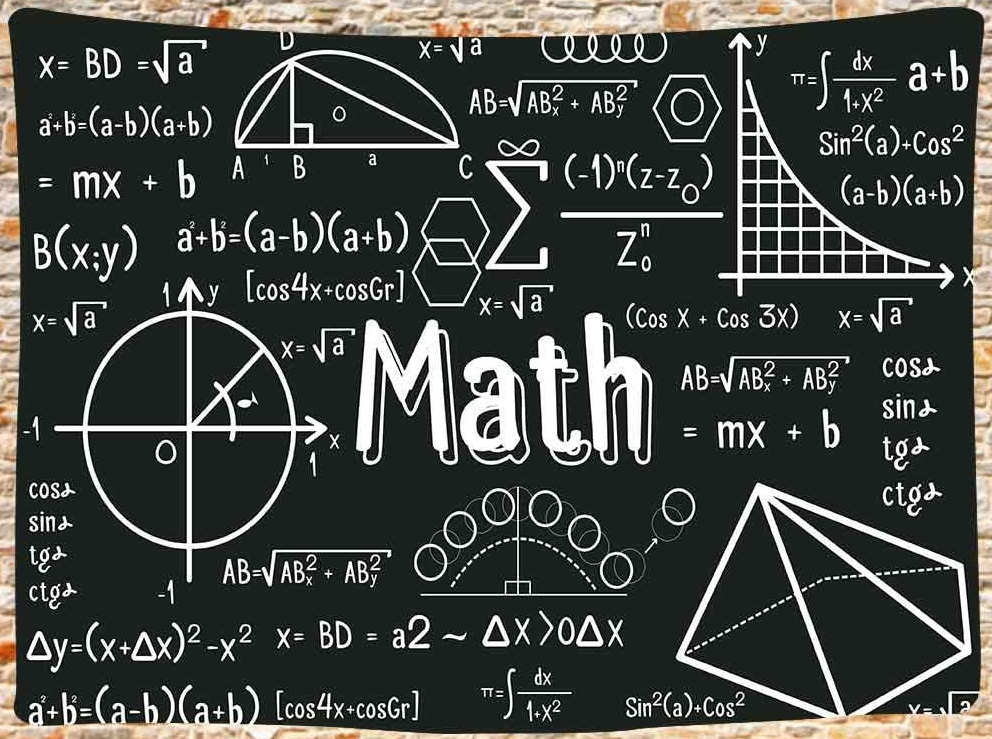
\includegraphics[scale=0.45]{images/math_p.png}
\end{center}
\end{document}